\documentclass{beamer}

\usepackage{listings}

\lstset{
    basicstyle=\small\ttfamily,
    breaklines=true,
    columns=fullflexible,
    frame=single,
    numbers=left,
    numberstyle=\tiny,
    language=C
}

\title{Le pseudo-terminal sur Linux}
\author{Oumar Magomadov}
\institute{École Supérieure d'Informatique}
\date{2023}

\usetheme{Warsaw}
\titlegraphic{
\includegraphics[width=2cm]{images/logo_esi.png}}

\begin{document}

\frame{\titlepage}

\begin{frame}{Table des matières}
	\frametitle{Table des matières}
	\tableofcontents
\end{frame}

% =================
\section{Introduction}

\begin{frame}

	\begin{itemize}[<+->]
		\item L'apparition d'un ordinateur central capable d'effectuer des opérations complexes
		\item Initié dans le domaine de la \textbf{recherche} et adopté par \textbf{le gouvernement}.
		\item Plus tard, son utilisation s'est étendue aux \textbf{entreprises}.
	\end{itemize}

\end{frame}

\begin{frame}

	\begin{itemize}[<+->]
			\item La nécessité d'un périphérique capable d'envoyer des instructions et de recevoir une réponse était cruciale à l'époque

			\item Un périphérique physique était souvent connecté à l'unité centrale via un port série, tel que \textbf{COM1}

				\begin{figure}
					\centering
					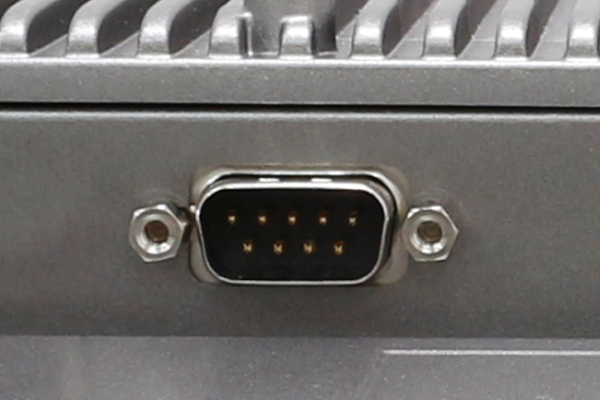
\includegraphics[width=3cm]{images/com1_serial.jpg}
					\caption{Un port série COM1}
				\end{figure}

			\item À cette époque, un ordinateur central était considéré comme un \textit{"réseau de terminaux"}
	\end{itemize}


\end{frame}

\begin{frame}

	\begin{itemize}[<+->]
		\item Le périphérique physique utilisé à l'époque était communément appelé un \textbf{terminal}.
		\item Un exemple bien connu de terminal physique était le \textbf{VT100}.

			\begin{figure}
				\centering
				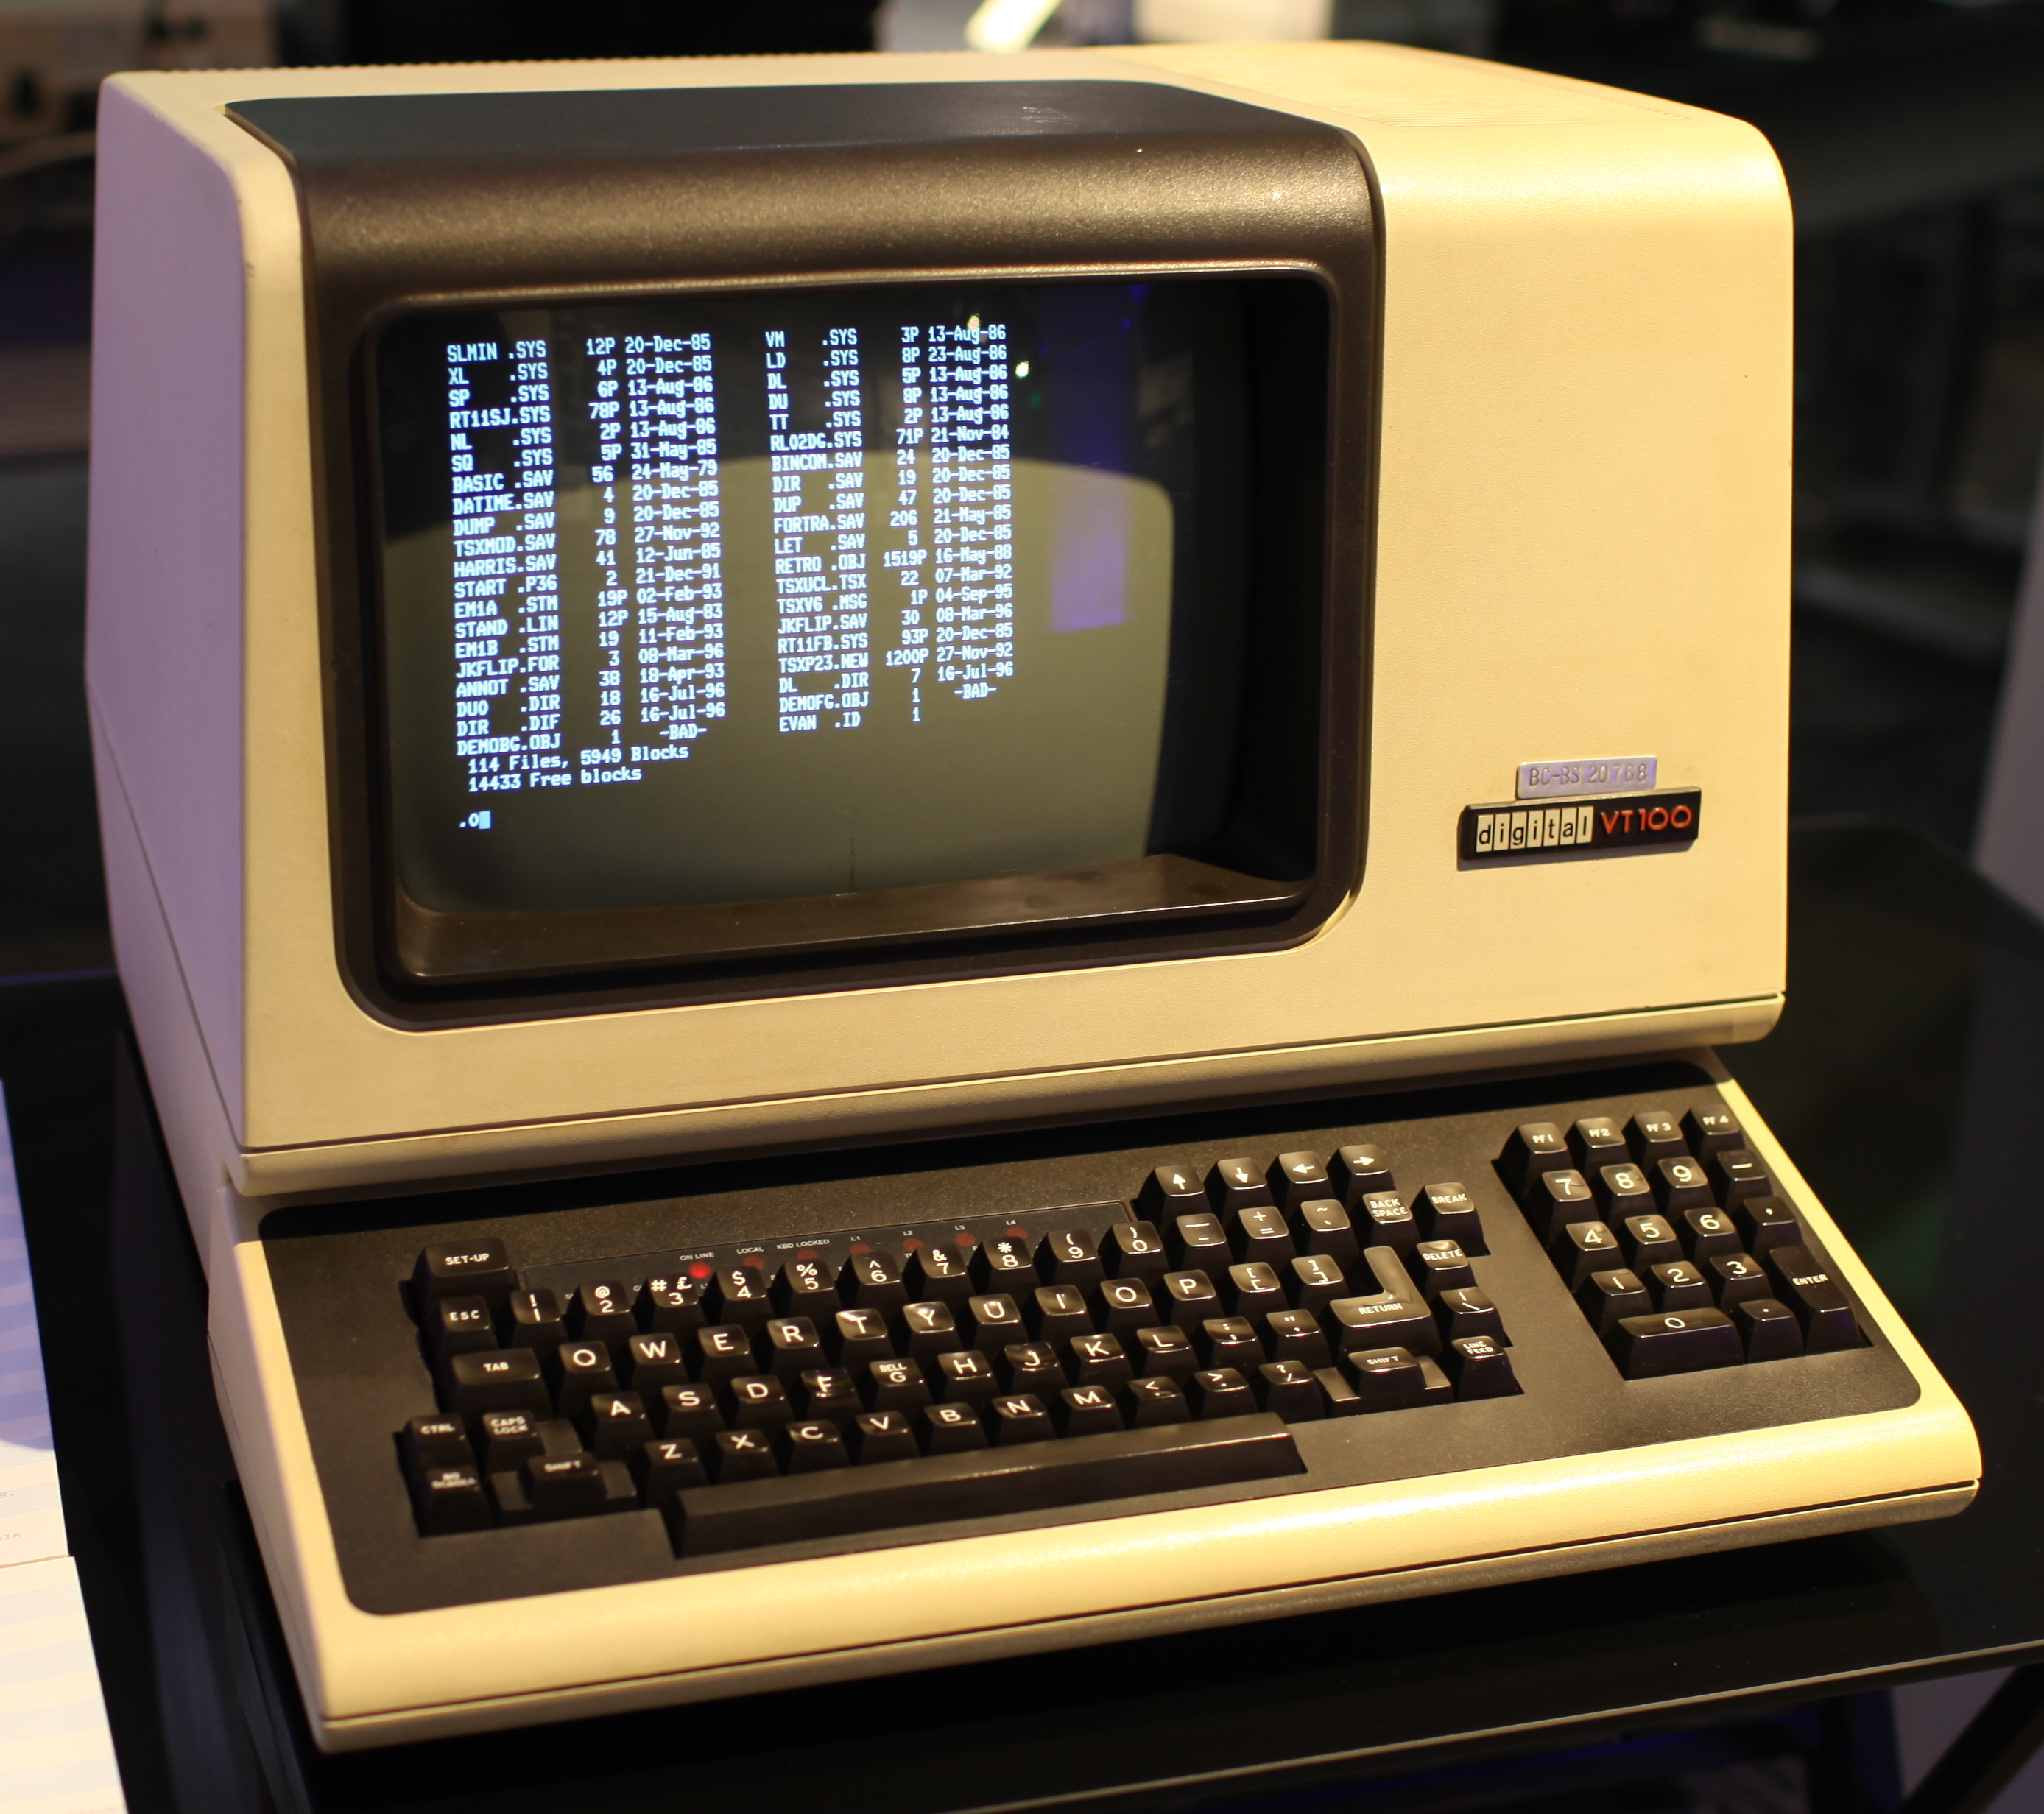
\includegraphics[width=4cm]{images/DEC_VT100_terminal.jpg}
				\caption{Un terminal physique DEC VT100 avec écran et clavier.}
			\end{figure}

		\item Les utilisateurs pouvaient accéder aux ressources de l'unité centrale à partir du terminal physique.
	\end{itemize}

\end{frame}

\section{Le terminal virtuelle}

\begin{frame}

	\begin{itemize}[<+->]
		\item L'apparition des ordinateurs personnels
			\begin{figure}
				\centering
				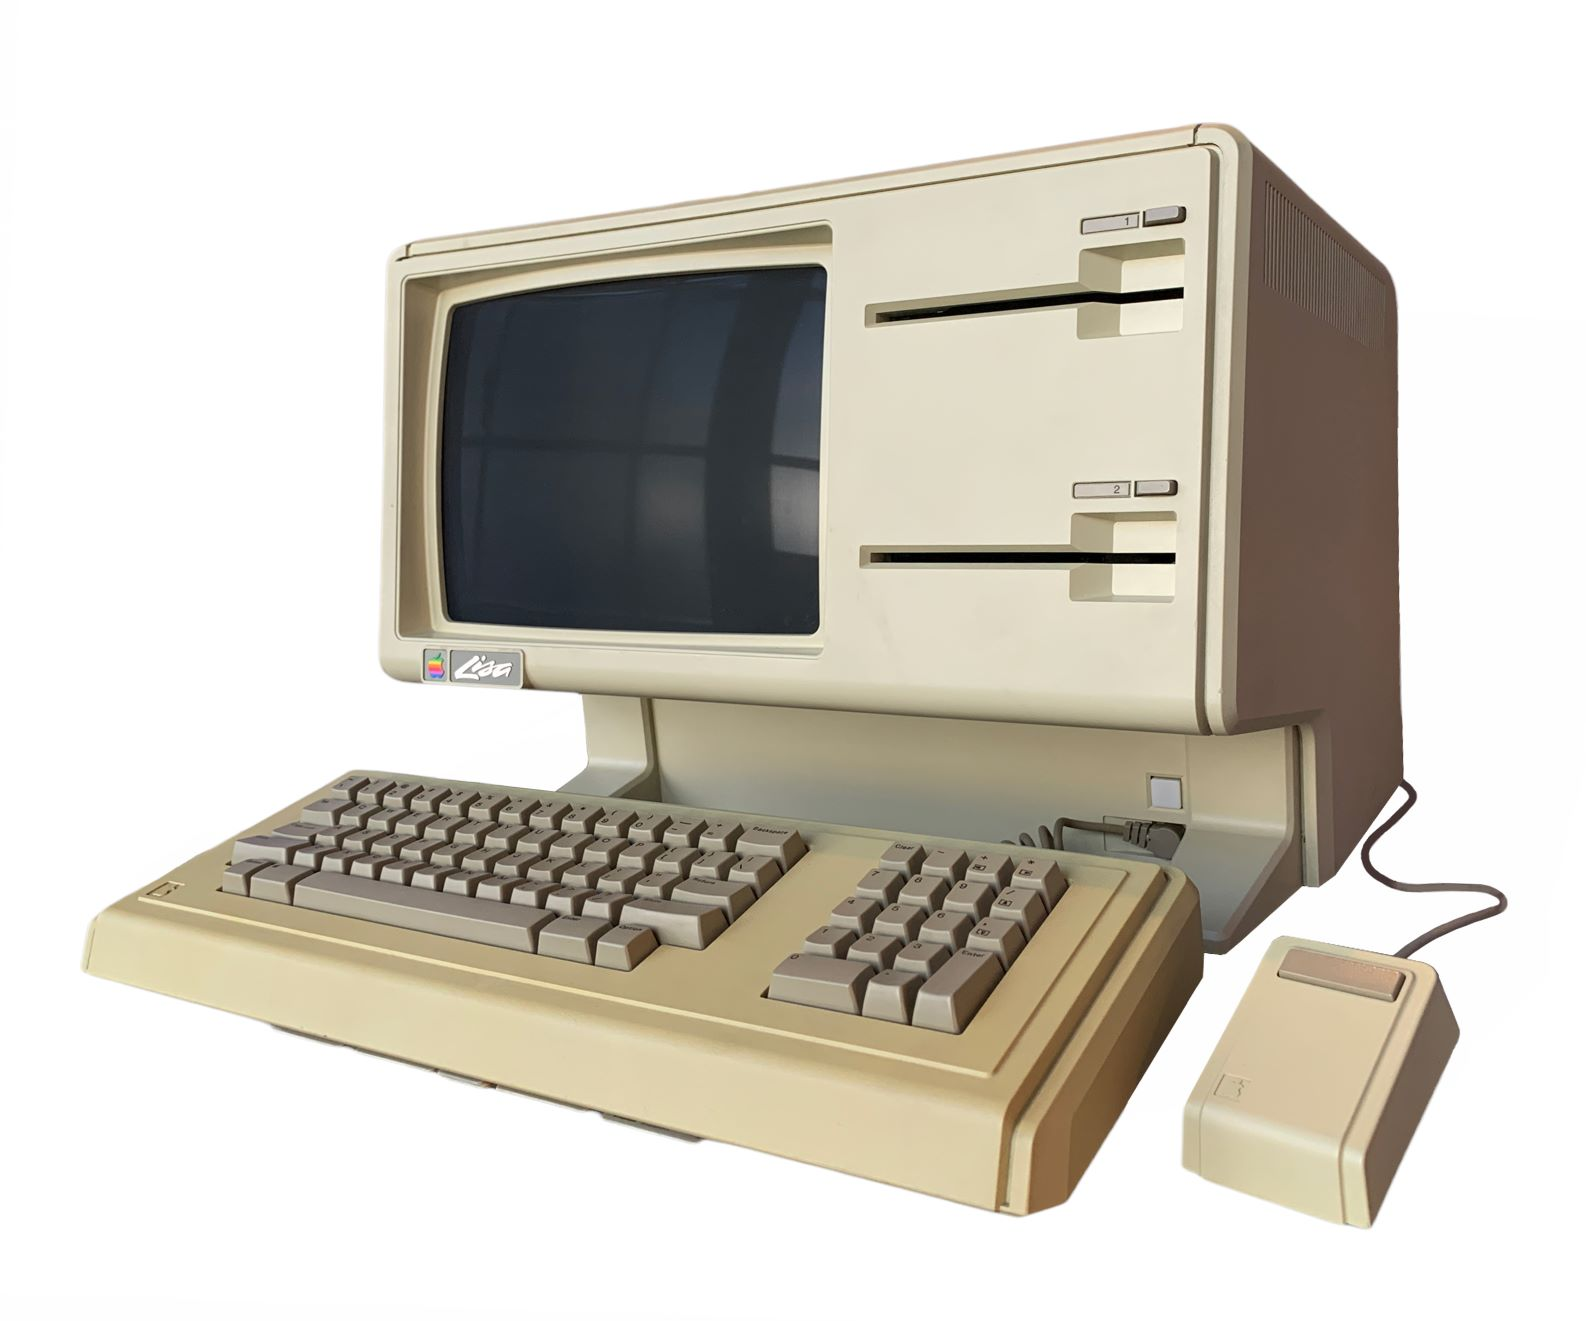
\includegraphics[width=4cm]{images/apple_lisa.jpg}
				\caption{Un ordinateur personnel surnommé "Lisa" créé par Apple.}
			\end{figure}

		\item Il n'était plus nécessaire d'utiliser l'unité centrale pour effectuer des calculs informatiques

		\item Les terminaux physiques sont utilisés de moins en moins
	\end{itemize}

\end{frame}

\begin{frame}

	\begin{itemize}[<+->]
		\item Utilisation d'interfaces en mode texte sur les ordinateurs personnels
		
		\item Quelques années plus tard, l'avènement des terminaux virtuels
		
		\item Possibilité d'ouvrir plusieurs sessions sur les consoles virtuelles
	\end{itemize}

\end{frame}

\begin{frame}

	\begin{itemize}[<+->]
		\item Offre une interface textuelle pour \textbf{interagir} avec le système d'exploitation
			\begin{figure}
				\centering
				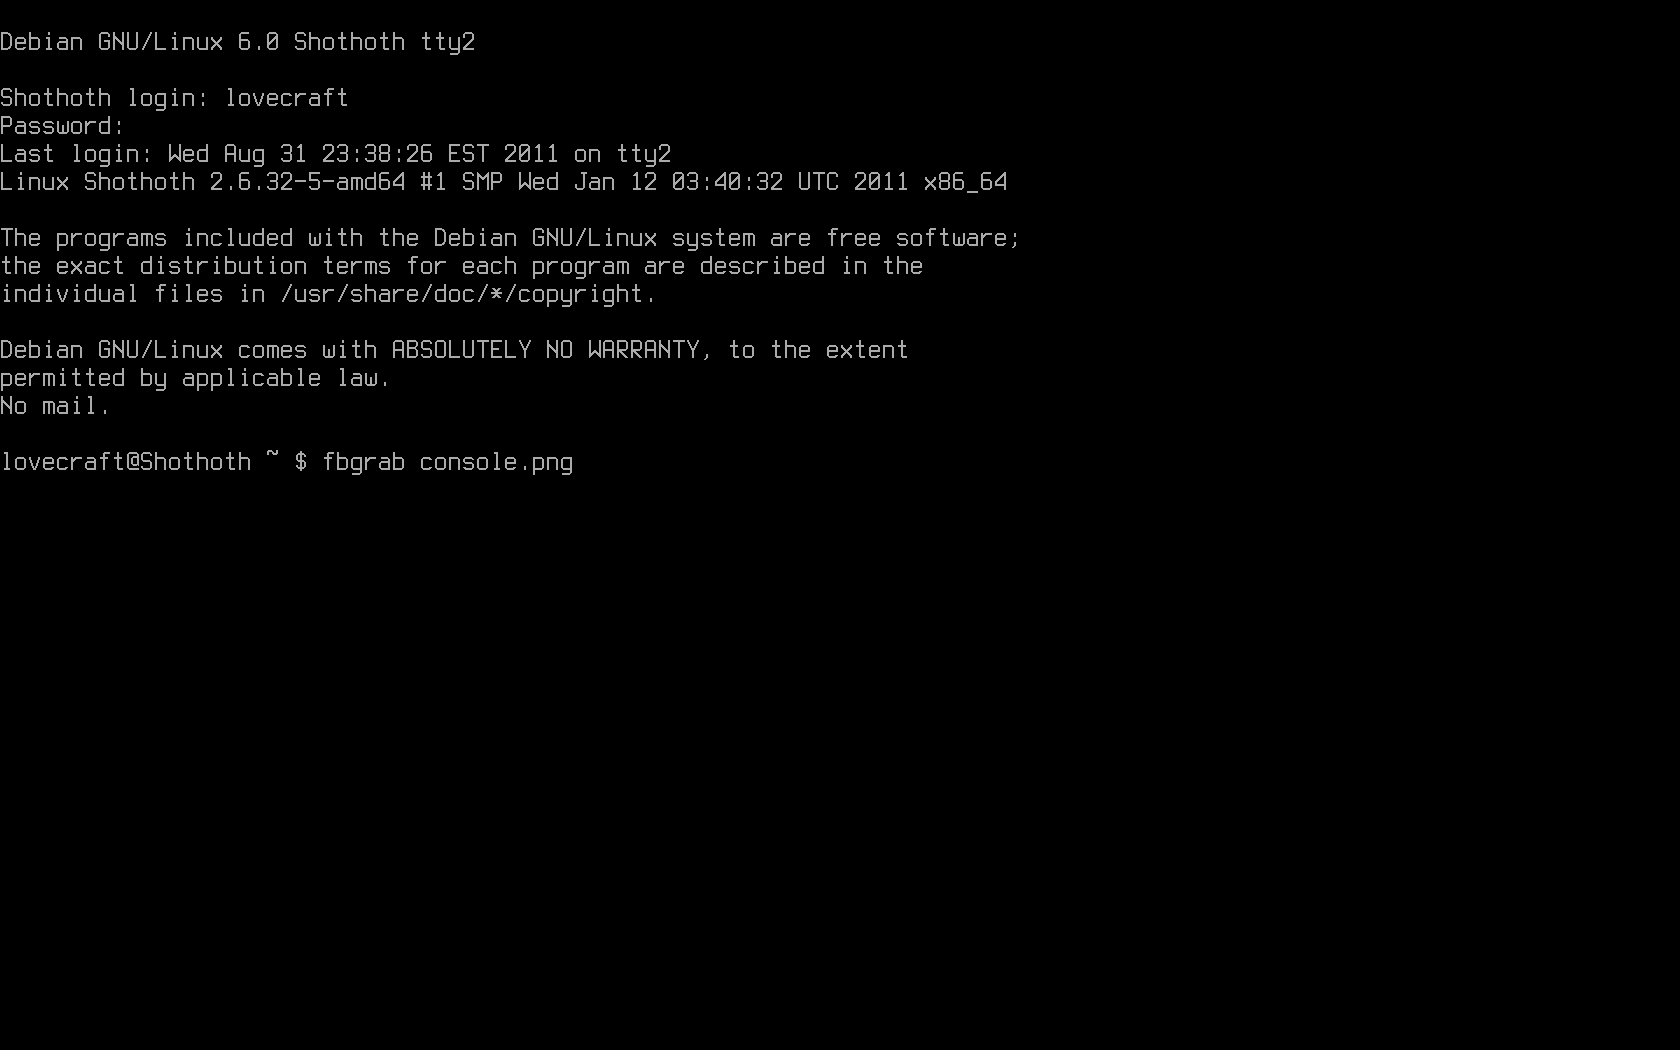
\includegraphics[width=5cm]{images/virtual_console.png}
				\caption{L'affichage d'une console virtuelle}
			\end{figure}
		\item Reçoit les entrées de l'utilisateur et affiche les résultats à l'écran

		\item Fonctionne de manière similaire à un \textbf{terminal physique}

	\end{itemize}

\end{frame}

\begin{frame}

	\begin{itemize}[<+->]

		\item Un répertoire spécial représentant les périphériques sous forme de fichiers

		\item Le répertoire \textbf{/dev} sur Linux/Unix
               
		\item Deux types de périphériques : \textit{caractère} \& \textit{bloc}
               
		\item Un terminal virtuel est un périphérique de type \textit{caractère}

	\end{itemize}

	\begin{block}{Quel est la différence}
		\begin{itemize}
			\item Un périphérique de type \textit{caractère} envoie \& reçoit des données sous forme de bytes
			\item Un périphétique de type \textit{block} envoie \& reçoit des données sous forme de blocs de bytes
		\end{itemize}
	\end{block}

\end{frame}

\begin{frame}	
	\begin{itemize}[<+->]
		\item Pour chaque périphérique, il y a un \textit{pilote}
        
		\item Un \textit{pilote} est essentiel pour le bon fonctionnement du périphérique
        
		\item Le terminal virtuel possède lui aussi un pilote appelé : \textbf{pilote de terminal}
	\end{itemize}

\end{frame}

\begin{frame}
	\begin{itemize}[<+->]
		\item Le \textbf{pilote de terminal} possède 2 tampons pour stocker des données

		\item Un tampon d'entrée appelé: \textit{input buffer}

		\item Un tampon de sortie appelé: \textit{output buffer}

	\end{itemize}

	\begin{block}{Une taille fixe pour le tampon d'entrée}
		Le tampon d'entrée possède une taille fixe définie par l'OS, généralement de \textit{4096 octets}. Il est impossible d'ajouter des données au-delà de cette taille.
	\end{block}
\end{frame}

\begin{frame}
	\begin{itemize}[<+->]
		\item Les entrées au clavier sont réceptionnées par le pilote du clavier et renvoyées pour traitement à l'OS
		\item Le \textbf{pilote de terminal} stocke les données reçues dans un tampon de taille fixe
		\item Les données sont traitées pour détecter tout caractère spécial

\item Le processus \textit{lecteur} effectue une lecture sur le tampon pour récupérer les données

\item Les données venant du processus \textit{lecteur} sont stockées dans un autre tampon
	\end{itemize}
\end{frame}

\begin{frame}
	\begin{itemize}[<+->]
		\item Le \textbf{pilote de terminal} peut être en mode \textit{canonique} ou \textit{non-canonique}
			\begin{figure}
				\centering
				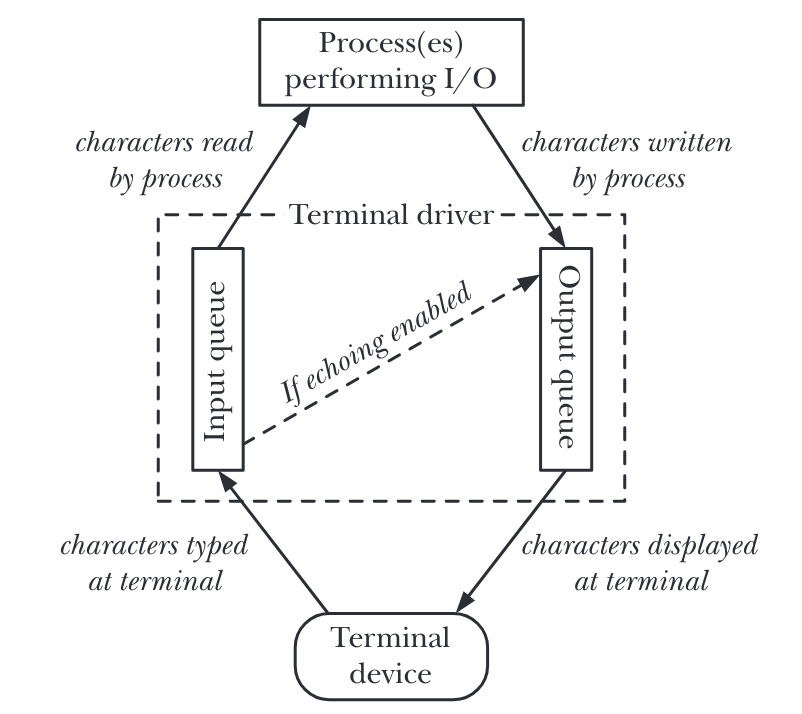
\includegraphics[width=4cm]{images/input_output_queue.png}
				\caption{Le schèma représentant les 2 tampons}
			\end{figure}
		\item En mode \textit{canonique}, les données sont stockées par ligne
		
		\item En mode \textit{non-canonique}, les données sont stockées par octets
	\end{itemize}
\end{frame}

\begin{frame}
	\begin{itemize}[<+->]
		\item Prise en charge des caractères spéciaux en mode canonique

		\item La touche \textit{Entrée} génère un caractère spécial \textbf{EOF}

		\item Des combinaisons de touches génèrent aussi des caractères spéciaux

	\end{itemize}

	\begin{examples}
		\begin{itemize}[<+->]
			\item Une fois que les données sont entrées par l'utilisateur et que celui-ci presse la touche \textit{Entrée}, un caractère spécial \textbf{EOF} à la fin de la ligne avertit le processus \textit{lecteur} qu'une lecture peut être effectuée.
			\item Le fait d'appuyer sur une combinaison de touches \textit{CTRL+C} génère un signal \textit{INTR} sur tous les processus tournant en \textbf{foreground}.
		\end{itemize}
	\end{examples}
\end{frame}

\begin{frame}
	\begin{itemize}[<+->]
		\item En mode non-canonique, les caractères spéciaux ne sont pas pris en compte.
		
		\item Le \textit{line editing} n'est également pas possible

		\item Le processus \textit{lecteur} lit directement les octets stockés dans le tampon.
	\end{itemize}
\end{frame}

\section{Le pseudo-terminal}

\begin{frame}
	\begin{itemize}
		\item Permet une \textbf{communication asynchrone} et \textbf{bidirectionnelle} entre deux processus
		\item Une extrémité \textbf{maître} et une autre extrémité \textbf{esclave}
		
		\item Utilisé par les émulateurs de terminal, tels que \textit{konsole} sur KDE

		\item C'est le noyau qui se charge de la création des pseudo-terminaux

	\end{itemize}

	\begin{figure}
		\centering
		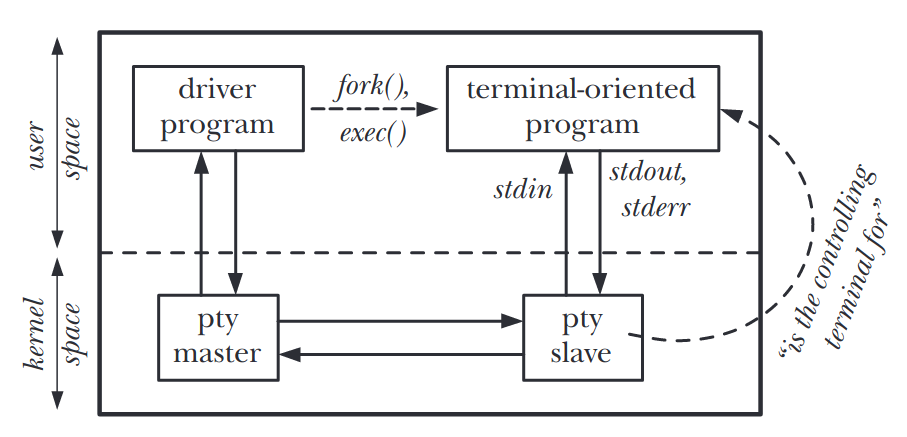
\includegraphics[width=5cm]{images/pseudo-terminal.png}
		\caption{Le fonctionnement du pseudo-terminal}
	\end{figure}
\end{frame}

\begin{frame}
	\begin{itemize}
		\item Un \textit{terminal de contrôle} pour les processus en \textit{foreground}

		\item Il gère les entrées, sorties et \textit{jobs} pour les pseudo-terminaux

		\item Une combinaison de touches permet de faire passer un processus en \textit{background}

			\begin{block}{Passer un processus en \textit{background}}
				Lorsqu'un processus s'exécute dans le shell Bash, on peut le basculer en arrière-plan en utilisant les touches \textit{CTRL+Z}. Pendant ce temps, le terminal reste disponible pour lancer d'autres commandes. Cette fonction est particulièrement utile pour des processus impliquant des tâches très longues.
			\end{block}
	\end{itemize}
\end{frame}

\begin{frame}
	\begin{itemize}
		\item Les processus se trouvent dans des \textit{sessions}
		\item Chaque session possède des groupes qui contiennent des processus
		\item Le groupes de processus dite \textit{foreground} détiennent le \textit{terminal de contrôle}
			\begin{figure}
				\centering
				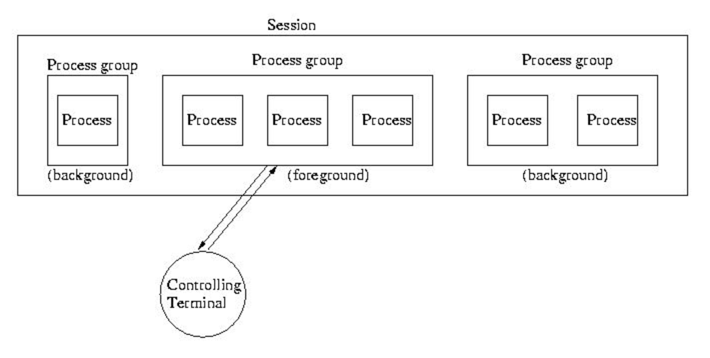
\includegraphics[width=6cm]{images/controlling_terminal.png}
				\caption{Les sessions \& groupes de processus sur Linux}
			\end{figure}
	\end{itemize}
\end{frame}

\section{Mise en pratique}

\begin{frame}[fragile]
	\textbf{Pour lire les données depuis le pseudo-terminal esclave}
	\begin{itemize}
		\item Effectuer une ouverture en lecture seul sur le fichier spéciale du pseudo-terminal esclave dans le répertoire \textbf{/dev}
		\item Avec ce descripteur de fichier, il sera possible d'effectuer \textit{read}
	\end{itemize}

	\begin{lstlisting}[language=C]
	if( (fd = open(path, O_RDONLY)) < 0 ) {
		perror("open");
		exit(EXIT_FAILURE);
	}
	\end{lstlisting}
\end{frame}

\begin{frame}[fragile]

	\begin{itemize}
		\item Le fait de lire sur le descripteur de fichier peut effectuer un \textit{blocage}
		\item Pour évité ça, utilisation de l'appel système \textbf{select()}
		\item \textbf{select()} permet de faire du monitoring sur des descripteurs de fichiers
		\item \textbf{select()} utilise pour ça 2 ensembles : readsfds \& writefds
		\item Il faut \textit{nettoyer} l'ensemble \& ajouter le descripteur dans l'ensemble
	\end{itemize}

	\begin{lstlisting}[language=C]
        FD_ZERO(&readfds);
        FD_SET(fd, &readfds);
        \end{lstlisting}
\end{frame}

\begin{frame}[fragile]

	\begin{itemize}
		\item \textbf{select()} retourne le nombres de descripteurs qui demandent une lecture ou écriture
		\item Effectuer un \textit{read} sur le tampon d'entrée
	\end{itemize}

	\begin{lstlisting}[language=C]
	while( (select(fd + 1, &readfds, NULL, NULL, NULL)) > 0 && strncmp("q", bytes, 1) != 0) {
                read(fd, bytes, 1);
                write(1, bytes, sizeof(bytes));
                FD_ZERO(&readfds);
                FD_SET(fd, &readfds);
        }
	\end{lstlisting}

\end{frame}

\begin{frame}[fragile]
	\textbf{Pour écrire des données sur le pseudo-terminal esclave}
	\begin{itemize}
		\item Effectuer une écriture seul sur le fichier spéciale du pseudo-terminal esclave dans le répertoire \textbf{/dev}
	\end{itemize}

	\begin{lstlisting}[language=C]
	if( (fd = open(path, O_WRONLY)) < 0 ) {
                perror("open");
                exit(EXIT_FAILURE);
        }
	\end{lstlisting}
\end{frame}

\begin{frame}[fragile]
	\begin{itemize}
		\item Utilisation de l'appel système \textbf{ioctl()}
		\item Permet de manipuler les paramètres d'un fichier spéciale de type caractère sur Linux
		\item Le pseudo-terminal esclave est bien un fichier spéciale de type caractère
		\item la commande \textbf{TIOCSTI} permet d'envoyer des bytes dans le tampon d'entrée du pseudo-terminal esclave
	\end{itemize}

	\begin{lstlisting}[language=C]
	while( (select(fd + 1, NULL, &writefds, NULL, NULL)) > 0 && ((messg = getchar()) != 'q') ) {
                if(ioctl(fd, TIOCSTI, &messg)) {
                        perror("ioctl");
                        exit(EXIT_FAILURE);
                }

                FD_ZERO(&writefds);
                FD_SET(fd, &writefds);
        }
	\end{lstlisting}
\end{frame}

% ================

\end{document}
